\documentclass{standalone}
\usepackage{tikz}
\usepackage{ctex,siunitx}
\setCJKmainfont{Noto Serif CJK SC}
\usepackage{tkz-euclide}
\usepackage{amsmath}
\usetikzlibrary{patterns, calc,3d}
\usetikzlibrary {decorations.pathmorphing,decorations.pathreplacing,decorations.shapes}
\begin{document}
\small
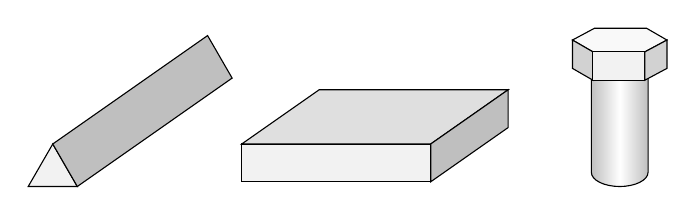
\begin{tikzpicture}[>=latex,scale=1.2]
  \begin{scope}
    \draw[fill=lightgray!20](90:0.3)--(-30:0.3)--(-150:0.3)--cycle;
    \draw[fill=lightgray](90:0.3)--++(35:2)--++(-60:{0.3*sqrt(3)})--++(35:-2)--cycle;
  \end{scope}
  \begin{scope}[xshift=3cm]
    \draw[fill=lightgray!20](-1,-0.1)rectangle(1,0.3);
    \draw[fill=lightgray!50](-1,0.3)--++(35:1.0)--++(2,0)--++(35:-1.0)--cycle;
    \draw[fill=lightgray](1,0.3)--++(35:1.0)--++(0,-0.4)--++(35:-1)--cycle;
  \end{scope}
  \begin{scope}[xshift=6cm]
    \draw[left color=lightgray,right color=lightgray,middle color=white](-0.3,0)arc(180:360:0.3 and 0.15)--++(0,1.2)--++(-0.6,0)--cycle;
    \draw[fill=lightgray!10](-0.5,1.4)--++(-30:0.25)--++(0:0.55)coordinate(a)--(0.5,1.4)--++(150:0.25)--++(-0.55,0)--cycle;
    \draw[fill=lightgray!70](-0.5,1.4)--++(0,-0.3)--++(-30:0.25)--++(0,0.3)--cycle;
    \draw[fill=lightgray!20]([shift=(-30:0.25)]-0.5,1.4)--++(0,-0.3)--++(0:0.55)--++(0,0.3)--cycle;
    \draw[fill=lightgray!70](0.5,1.4)--++(0,-0.3)--([shift=(-90:0.3)]a)--++(0,0.3)--cycle;
  \end{scope}
\end{tikzpicture}
\end{document}